For python GUI development wxPython was a great choice because it offered simplicity and progress was easy.
The framework supports loose coupling and high cohesion, it gives the opportunity to develop separate components
and combine them later. This design feature was used to develop a component for each set of elements in the
wireframe \ref{guie}. 

\begin{figure}[htp]
\centering
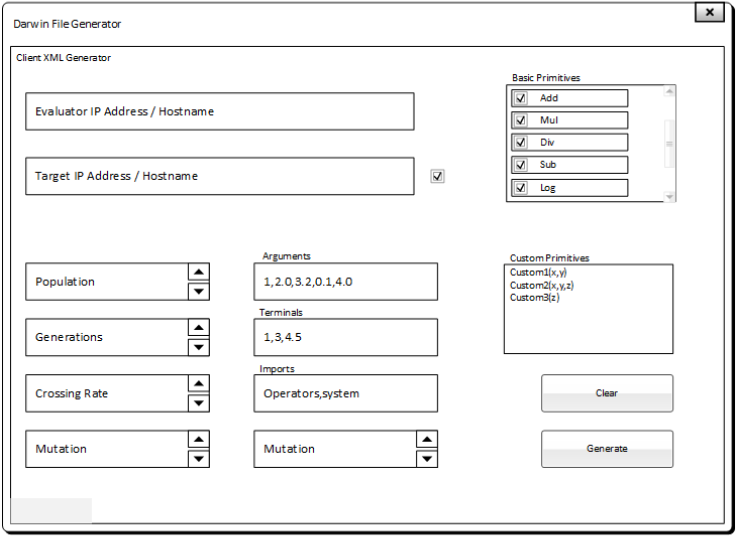
\includegraphics[scale=0.6]{Figures/guiit.png}
\caption{One of the iterations of the GUI showing all the possible parameters}
\label{fig:guie}
\end{figure}

The GUI was split into five components \ref{guicode}.

\begin{enumerate}
	\item \textit{InitMenu()} initializes the menubar on top, creates each of the menu and sub-menu options and 
	handles the functionality of the menu items.
	\item \textit{InitTexts()} creates a pane that has text input fields for the URLs of the target web service and 
	the evaluator.
	\item \textit{InitAttributes()} returns a pane that has fields that specify the parameters used in the genetic program (e.g. crossing rate, mutation rate, population size, number of generations)
	\item \textit{InitPrimitives()} creates a primitives selector. The selector is created by combining several wxPython components like \textit{scrollable panes}, \textit{CheckListControl} and multiple
	sizers to organize the buttons and create a better feel.
	\item \textit{InitButtons()} simply creates a plane with the button \textit{Generate} however it would be expected that later on more buttons would be added
\end{enumerate} 

\begin{lstlisting}[language=Python,caption={The method in the GUI that initializes all the components used},label={lst:guicode}]

def InitUI(self):
    self.InitMenu()
    textPanel = self.InitTexts()
    attrPanel = self.InitAttributes()
    primPanel = self.InitPrimitives()
    buttPanel = self.InitButtons()
\end{lstlisting}

When the \textit{Generate} button is pressed the UI is organizing all the data from the fields into a dictionary which is passed to the XML parser to generate the XML configuration file.
